\chapter{Trajectory Planning}

The main task of this thesis is to solve the problem of trajectory planning for a fast moving car. In this chapter, we will analyze this problem in depth. We will first look into the planning problem in general and then we will discuss what the term ``fast moving cars'' means and how trajectory planning for a fast car is different from the general problem.

With the knowledge of the theory, we will formulate our trajectory planning problem. We will consider several well-known search algorithms used to solve planning problems and adapt them to our problem.

The solution of the planning problem will be a reference state trajectory. The vehicle will try to follow this trajectory as closely as possible using a different algorithm as it was shown in Figure~\ref{fig:racing_agent_diagram}. The state trajectory will include both a path the vehicle should follow and a speed profile. Using this information, our vehicle will be able to go through corners efficiently by slowing down and accelerating at convenient times and by following an appropriate racing line.

\section{Introduction to Planning}

\subsection{Automatic Planning}

The world of a planning problem is defined in terms of states and actions. A single state is a full description of the important aspects of the environment and it is usually encoded as a vector of (real) numbers. All of the possible states of the world form a state space. An action is a way of changing the current state of the world into a different state. The planning task is to find a sequence of actions, which changes the state of the world from a given initial state to some desired state, called a goal state. This sequence of actions is referred to as a feasible plan.

With the intuition of what a planning problem is, we can formulate it formally. We will state a generalized definition based on the definitions given in the book \textit{Planning Algorithms} \cite{lavalle_2006}:

\begin{defn}[Planning Problem]
	\label{def:basic_planning_problem}
	A planning problem is a tuple $\left(X, U, f, x_0, X_g\right)$ consisting of:
	
	\begin{enumerate}
		\item A \textit{nonempty set} $X$ of world states, called the \textit{state space}.
		\item For each state $x\in X$, a set of actions $U(x)$, called the \textit{action space}.
		\item A \textit{state transition function} $f$ defined for every $x\in X$ and $u\in U(x)$, which produces the state of the world after applying the action $u$ to the state $x$.
		\item An \textit{initial state} of the world $x_0\in X$.
		\item A \textit{nonempty set} of goal states $X_g\subset X$.
	\end{enumerate}
\end{defn}

\begin{defn}[Feasible Plan]
	A solution to a planning problem $\left(X, U, f, x_0, X_g\right)$ is feasible plan, which a finite sequence of actions $\langle u_0, u_1, \ldots, u_k\rangle$ such that:
	
	\[
		\forall i \in \left\{0,1,\ldots,k\right\}: u_i\in U(x_i) \wedge x_{i+1}=f(x_i, u_i)\text{, } x_{k+1}\in X_g.
	\]
\end{defn}

\subsubsection{State Space Graph}

We can imagine that the states form vertices of a graph $G=(V, E)$ and the applications of actions through the state transition function form directed edges between the vertices:

\begin{equation*}
\begin{aligned}
	V&=X \\
	E&=\left\{(x_1, x_2) \mid \exists u \in U(x_1): x_2 = f(x_1, u) \right\}.
\end{aligned}
\end{equation*}

A feasible plan is then a directed path in the graph starting in the initial state vertex $x_0$ and ending in any of the goal states vertices. Finding a path in a graph is well-studied problem and there are several efficient algorithms to solve it, such as the Dijkstra algorithm or its extension called A*.

The size of the state space and the action spaces has great impact on the way how we approach the planning problem and how we find a solution. If the graph is finite or if the the number of vertices is countably infinite and the branching factor is finite, we can still find the solution (if one exists) with a systematic search algorithm in a finite amount of time. If no solution exists, the algorithm will be trying different plans infinitely, unless there is a limiting criterion, such as maximum length of a plan.

When the number of vertices becomes uncountably infinite or the branching factor is infinite, the problem becomes harder and we cannot rely on a simple graph search anymore. We will soon see, that the state space of all of the vehicle configurations in our problem is uncountably infinite. We will have to overcome this problem in order to find a practical representation which can be used in practice on a robot.

Even though we transformed planning into a well-known problem of graph search, we must keep in mind that the number of states of the system can be very high even if it is finite. Because the state space represents all of the combinations of the state variables of the world. 

\subsection{Planning Under Differential Constraints}
\label{sec:planning_under_differential_constraints}

When describing the motion of a car-like robot on a two-dimensional plane, the configuration of the body of the vehicle is described by at least the pose of the vehicle, which consists of three variables: the $x$ and $y$ Cartesian coordinates of some reference point of the body of the vehicle, and the angle $\theta$ in which the heading angle of the robot  (an angle between the longitudinal axis of the vehicle and the $x$ axis). The $(x, y)$ location is usually in some area $P\subseteq\mathbb{R}^2$ and the heading angle is an arbitrary angle $\theta\in\left[0,2\pi\right)$. This simple configuration space has three continuous dimensions and it is infinite. The robot does not jump from one pose to another, but its configuration can be described as a continuous path through the configuration space over time. The kinematics and dynamics of a robots are usually described by differential equations. These equations give us the velocities at which the state of the robot moves through the configuration space.

As an example of these constraints, we can look at a model of a \textit{simple car} shown in the book \textit{Planning Algorithms} by Steven M. LaValle \cite[Section~13.1.2.1]{lavalle_2006}. The state space consists of the poses in a 2D plane $(x, y, \theta)$ as we described it earlier. The control inputs are two dimensional vectors $\left(u_s, u_\varphi\right)$, where $u_s$ is the commanded speed of the vehicle in the direction perpendicular to the rear axis, and $u_\varphi$ is the steering angle of the front wheels. For a better understanding of this example, see the Figure~\ref{fig:simple_car}. For a car with a wheelbase length $L\in\mathbb{R}$, its velocity can be approximated by this set of equations:

\begin{equation}
\begin{aligned}
\dot{x}&=u_s \cos \theta \\
\dot{y}&=u_s \sin \theta \\
\dot{\theta}&=\dfrac{u_s}{L} \tan u_\varphi.
\end{aligned}
\end{equation}

\begin{figure}
	\centering
	\label{fig:simple_car}
	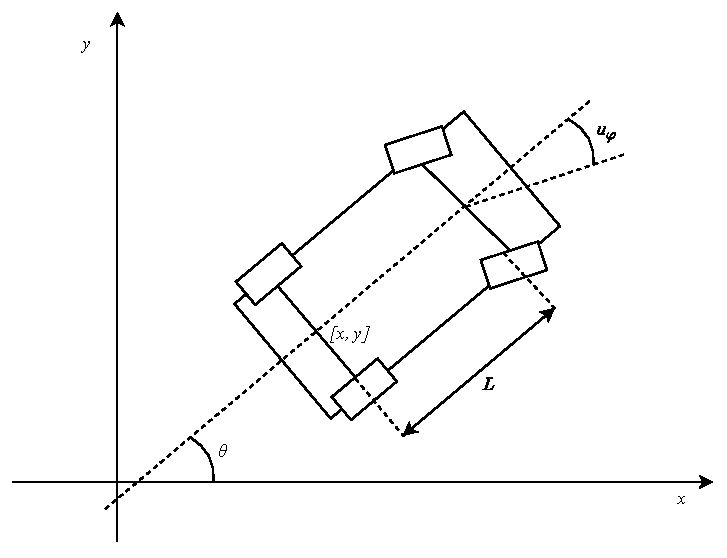
\includegraphics[width=12cm]{../img/simple_car.pdf}
	\caption{The simple car from the example has three state variables. The speed and the steering angle are action variables and they can change at any moment, so the vehicle can stop on a spot and change the steering angle instantaneously, which is of course not possible in a real world car.}
\end{figure}

In order to be able formulate the planning problem for a system with differential constraints, we must change the meaning of the \textit{state transition function} $f$ from how we defined it in Definition~\ref{def:basic_planning_problem}.

This function used to output the next state $x'$ after an action $u$ is applied to a state $x$, i.e. $x'=f(x, u)$. When the state space is continuous, the outcome of an execution of an action depends on for how long it is being applied. The state transition should now rather return the velocity in the configuration space:

\[
	\dot{x}=f(x, u).
\]

To predict the change of the sate after some time period $t\in(0,\infty)$, we must integrate the velocity. In order to be able to do that, we need to know which action is applied at any given moment of the time interval $T=[0, t]$ in a form of an \textit{action trajectory} $u: T \rightarrow U$, where $U=\bigcup\limits_{x\in X} U(x)$ and the action applied at time $t'$ is $u(t')$. We define the \textit{state trajectory} as $x: T \rightarrow X$, where $x(0)$ is the state at the end of the interval and $\forall t' \in T \setminus \left\{0\right\}$:

\[
	x(t')=x(0)+\int_{0}^{t'} f(x(\tau), u(\tau)) d\tau.
\]

\todo{Talk about sampling methods}

In the case when we are interested in how the state changes from the previous state $x(t)$ after a period $\Delta t$ of an execution of a constant action $u$ such that $\forall \tau \in \left[0, \Delta t\right]: u\in U(x(t + \tau))$, we can now define an discrete variant of the state transition function $f_{\Delta t}$ which behaves similarly to the original state transition function:

\[
f_{\Delta t}\left(x(t),u\right)=x(t+\Delta t)=x(t) + \int_{0}^{\Delta t} f\left(x(t+\tau),u \right) d\tau.
\]

\section{Trajectory Planning For Fast Moving Cars}

In this section we will discuss what it means to plan a trajectory for a fast moving car. What is the difference between trajectory planning for a slow moving car and for a fast moving car? What do we even consider to be a ``fast moving car'' and what is just a slow moving car?

A fast moving car is not a widely used term and it does not have a formal definition. Intuitively, we would consider a ``fast moving car'' to be a Formula 1, a rally car, or a different racing car. The racing drivers push their vehicles to their limits in order to be the first one behind the finish line. We might also consider ordinary driving on a motorway to be ``fast'', especially during a lane change maneuver or when we accelerate to overtake a vehicle in front of us. We might even consider driving at lower speeds to be ``fast'' when it involves taking sharp turns.

One thing these scenarios have in common is that the car reaches a speed at which it can become hard to steer the car in a specific direction because the tires might lose grip and the car might start moving sideways or in a more extreme scenario the car could roll over sideways. The speed which could be considered ``fast'' varies based on the radius of the turn.

For the purposes of this thesis, we will formulate the term in the following definitions:

\begin{defn}[Handling limits of a vehicle]
	We say, that a car is moving at its handling limits during a turn of a radius of $r\in(r_{min}, \infty]$ meters, if it is driving close to a speed $v_{max,r}$ at which the total force vector acting on the body of the vehicle would exceed the forces of the tires which keep the vehicle traveling at the constant radius $r$.
\end{defn}

The minimum turning radius $r_{min}\in\mathbb{R}$ is a constant specific for a given vehicle. It refers to the minimum turning radius which the vehicle can achieve at a very low speed and with the maximum steering angle possible. We can consider driving straight as driving along a circle with the radius of $\infty$ meters.

\begin{defn}[Fast moving car]\label{def:fast_moving_car}
	A car is moving fast when it is approaching its handling limits during a turn.
\end{defn}

\begin{defn}[Trajectory planning problem for a fast moving car]
	We say that a trajectory planning problem for a fast moving car is a planning problem under differential constraints, whose solution is a time-optimal state trajectory and the vehicle does not at any point in time exceed its handling limits.
\end{defn}

To achieve a time-optimal trajectory, we will search for a trade off between the length of the path and the speed at any given moment. To keep within the handling limits of the vehicle, our differential constraints must closely model the behavior of the vehicle. Even if our model of the vehicle describes its behavior well, it is more than likely that the robot will deviate from the planned trajectory at some point. The noise in sensor readings, imperfections in the actuators, or imprecise map of the track, all of these factors will contribute to errors in trajectory tracking. At some point, the difference between the planned path and velocity profile of the vehicle will be so large, that it will be advantageous to create a new plan from the current pose and speed of the vehicle. To make this possible, we need to be able to re-plan the trajectory in a short period of time.

Given our assumption, that we will most likely have to re-plan the trajectory at some point in the future anyway, it does not make too much sense to plan the trajectory for the whole circuit at once. The longer the trajectory we are planning, the longer it will take to find a suitable plan. Instead, we could split the track into multiple shorter segments and plan a trajectory only for a few of the segments directly in front of the current pose of the vehicle.

When the vehicle is moving fast, a late or too early decision to change the direction or adjust the speed of the vehicle might result in a crash or a sub-optimal trajectory. Fast reaction times are therefore key. If we plan a trajectory for only a limited stretch in front of the vehicle, we must be able to find the plan for the following stretch before we reach the end of the current reference trajectory. Failing to do this, the vehicle will not have any trajectory to follow and it would probably have to preform some kind of an emergency braking in order to prevent collisions, or it would be forced to resort to some simpler reactive steering strategy, which does not involve planning ahead and which would most likely be sub-optimal.

We can now summarize the discussion in this section into a set of requirements for the trajectory planning algorithm which will make it more suitable for fast moving cars:

\begin{itemize}
	\item The whole track should be split into smaller segments, so that we do not have to waste resources to plan a trajectory for segments which will most likely not be reached by the time we will need to re-plan the trajectory.
	\item The differential constraints of the vehicle must accurately describe capture the movement of the vehicle at its handling limits and we must be able to eliminate dangerous maneuvers, which could lead to a crash or a trajectory or which could not be followed closely by the vehicle.
	\item The search algorithm we will use must find good solutions which are time-optimal or close to time-optimal in a very short period of time.
\end{itemize}

\subsection{Problem Formulation}

\subsubsection{Coordinate System}

Our vehicle will move on a flat racing track. We can assume that there will not be any changes in the slope of the track and that we will not encounter any bridges or underpasses and that the wheels of our vehicle will always be in contact with the road surface.

We will use the common two-dimensional Cartesian coordinate system to represent the position of the global position of the vehicle on the track. The area of the track which is reachable by the vehicle is limited by the bounds of the racing track and so the set of all reachable positions of the track is $X\subseteq\mathbb{R}^2$.

\subsubsection{The Discrete-Time Model}

\todo{Describe delta T and refer to LaValle 14.2.2}

To obtain the next state of the vehicle, we need to integrate this derivative over some time interval $\Delta t > 0$ numerically. This time period must be chosen carefully to be as short as possible to minimize errors caused by numerical integration but at the same time long enough to decrease the computational load caused by frequent usage of the state transition function by the planning algorithm when exploring the state space. We must also consider the hardware limitations and the frequency with which we can change the input signal for the actuators.


\subsubsection{State Space}

Our state space $S$ will consists of all the possible configurations of the vehicle. The state space will be slightly different based on the vehicle model which is used in order to capture all the variables required by the model including the configuration of the chassis and the state of the actuators.

Independently of the choice of the vehicle model, the state will always contain the pose of the vehicle in the 2D coordinate space. By the pose of the vehicle we understand a tuple $\left( x, y, \theta\right)\in X\times \left[0, 2\pi\right)$, where $\left( x, y\right)$ are the coordinates of the center of gravity of the vehicle and $\theta$ is the angle between the $x$ axis of the coordinate system and the longitudinal axis of the vehicle, i.e. the heading angle of the vehicle.  The space of all vehicle poses is continuous and so the state space itself will always be continuous no matter what vehicle model we use. We will sometimes refer to the state space as the configuration space.

\paragraph{Initial State}
At the start of the race, the vehicle is expected to be situated at a predefined starting location of the racing circuit with its heading angle identical to the direction of the race. The vehicle starts from a standstill with the wheels not spinning and the front wheels pointing the heading direction of the car.

During the race, the speed and the steering angle have to be measured using sensors. We must take in mind that this state is most likely slightly inaccurate due to the errors in the measurements and due to a delay between the measurement and the start of planning. By the time the planning algorithm finds a trajectory, the state vehicle will have already changed and it will be different from the initial conditions of the planning algorithm.

\subsubsection{Collision Detection}

\subsubsection{Action Space}

As we discussed earlier, our vehicle has two actuators which we can control:
\begin{itemize}
	\item Steering servo which we can move to a desired position achieving a specific steering angle between the maximum left position, center position, and maximum rotation to the right.
	
	\item Motor which can be set to a specific \gls{RPM} and a direction of rotation when there is no load. The \gls*{RPM} will differ based on the load of the vehicle and the motor will require more voltage to achieve some RPM when the load is increased.
\end{itemize}

The electric signal we send to the actuators is interpreted as a target value and the actuator adjusts its output to match the target value over a time period at a rate which we cannot control. We define the action space for these actuators like this:

\[
U=\left\{ \left( \delta_t,\tau_t\right) \mid \delta_t,\tau_t\in\left[-1, 1\right] \right\}
\]

$U$ is a set of tuples of a steering angle proportion $\delta_t$, and a throttle position $\tau_t$. These actions are an abstraction of the signals which would be to the hardware. Negative throttle position $\tau_t$ means that the motor should spin in reverse, while positive values should result in the motor spinning in the normal direction of travel. When the vehicle is moving in some direction and the action specifies a throttle position in the opposite direction, the vehicle might engage brakes, if it is equipped with any.

Since these actions represent merely the target values of the state of the actuators, our actions do not have any preconditions for the state in which they can be executed. On the other hand, executing some actions for a given time period $\Delta t$ might result in a collision with an obstacle. To avoid this problem, we will limit the action set of a vehicle state by incorporating the collision detection function and the state transition function $f_{\Delta t}$ to allow only safe actions:

\[
	U(x)=\left\{u\in U \mid c(f_{\Delta t}(x, u)) = F\right\}.
\]

It is worth noting that if the vehicle is in state when its action set is empty, the vehicle is in a state when a collision within $\Delta t$ is inevitable.

The set $U$ as we defined it is infinite. In practice, our actuators can be set only to a fixed number of values. The \gls*{PWM} signal which controls the servo motors can only encode a finite number of levels. For a specific vehicle hardware, we can use only a finite subset $U_f\subset U$, $\abs{U_f}\in\mathbb{N}$ of valid actions.

\subsubsection{Goal Condition}

In Definition~\ref{def:basic_planning_problem} we used a set of goal states to check if a plan is a solution to the problem or not. \todo{Here I want to explain why we want waypoints}

\todo{rewrite this}

To ensure that our vehicle goes around the circuit in the correct direction and even in cases, when the track intersects itself and forms loops, we can place a finite sequence of waypoints along the track. An example of a circuit with waypoints can be seen in Figure 2: Racing circuit with a start/finish line and three way-points. 
We will require the vehicle to pass all the way points in the given order before we would consider the vehicle to finish a lap when it crosses the finish line.

Figure 2: Racing circuit with a start/finish line and three way-points.
For the sake of simplicity, we can treat all waypoints as circles of a given radius. We can also ignore the finishing line and instead use the first waypoint on the track as a target. This will force the vehicle to cross the finishing line without any need for modeling of the finish line itself. We do not want to stop at the finishing line anyway, because we should keep circling around the circuit if possible.

\begin{defn}
	Circular waypoint $\left(w,r\right)\in W$ is a tuple containing the location w and the radius $r$ of the waypoint.
\end{defn}

\begin{defn}[Waypoint]
	Waypoint goal region $G(w,r)=\left\{s\in S \mid \norm{X(s)-w}<r\right\}$ where $X(s)$ is the position vector of the state $s$, is a set of all states which are considered to pass the waypoint. The notation $\norm{\cdot}$ represents the Euclidean norm in $\mathbb{R}^2$.
\end{defn}
	
For our purposes it is not necessary to consider the state of the vehicle other than the position. We do not require the vehicle to be oriented in a specific direction or to come to a stop at the goal position.

\begin{defn}
	A sequence of states $\langle s_0,s_1,s_2,\ldots,s_k\rangle$ passes a sequence of waypoints $\langle \left(\vec{w_1}, r_1\right), \left(\vec{w_2}, r_2\right), \ldots, \left(\vec{w_l}, r_l\right) \rangle, l > 0$ when a sequence of indexes $\langle i_1,i_2,i_3, \ldots i_l \rangle$ exists such that:

	\begin{equation*}
		\begin{aligned}
			\forall m,n &\in \left\{1,\ldots,l\right\}: m<n\implies i_m < i_n \\
			\forall m &\in \left\{1,\ldots,l\right\}: s_{i_m}\in G(\vec{w_m}, r_m) \\
			i_l &= k \\
		\end{aligned}
	\end{equation*}
\end{defn}

\begin{defn}
	The goal condition $g_{\hat{w_l}}: S^* \rightarrow \left\{T,F\right\}$ is a function which for a given sequence of waypoints $\hat{w_l}$ and a state trajectory  $\hat{s_k}=\langle s_0,s_1,s_2,\ldots, s_k\rangle, k>0$ returns $T$ iff $\hat{s_k}$ passes $\hat{w_l}$.
\end{defn}
	
This goal condition definition gives us an ability to search for a state trajectory which is shorter than the whole lap. This is useful for searching a reference trajectory for only a few corners ahead and reduce the size of the searched portion of the state space. Motion planning in general is an NP-complete problem \cite[Section~6.5]{lavalle_2006} and it might not be possible to plan a reference trajectory for the whole circuit online especially for long circuits with many corners.

\todo{finish this}


\subsubsection{Problem Formulation}

In the previous sections, we described and defined the individual components of the trajectory planning problem. We can now formulate it formally:

\begin{defn}[Trajectory Planning Problem]

	A trajectory planning problem for a fast moving car is a tuple $\left(X, U_f, f_{\Delta t}, c, x_0, g_{\hat{w}}\right)$:

	\begin{itemize}
		\item A non-empty set $S\subseteq\mathbb{R}^n$, which is the state space of the vehicle. Each state of the vehicle is represented by $n\in\mathbb{N}:n\geq3$ state variables and it contains the pose of the vehicle in a two dimensional plane and other state variables as defined by the vehicle model which is used.

		\item A non-empty finite set $U_f$ of actions, such that $\forall x\in X, \forall u\in U_f(x): c(f_{\Delta t}(x, u)) = F$, where $c$ is a collision detection function.

		\item A state transition function $f_{\Delta t}:S\times U_f \rightarrow S$ for a fixed time period $\Delta t>0$.
		
		\item An initial state of the vehicle $s_0 \in S$.

		\item A goal condition function $g_{\hat{w}}: S^* \rightarrow \left\{ T, F\right\}$ for some fixed sequence of waypoints $\hat{w}=\langle w_0, \ldots, w_k \rangle$.
	\end{itemize}
\end{defn}

\subsubsection{Time-Optimal Feasible Solution}

The vehicle starts in an initial state $x_0$. It is controlled through an input sequence of actions applied over time at a constant rate, because we chose a fixed time interval $\Delta t>0$ between application of any two consequent actions. We can calculate the expected evolution of the state of the vehicle by integrating the velocity from a state transition function. If we take snapshots of the state every $\Delta t$ interval, we will get a sequence of states which we call a state trajectory:

\begin{defn}[Feasible State Trajectory]
	We say that a sequence of states $\hat{x_k}=\langle x_0,x_1,x_2,…,x_k \rangle ,x_i\in X$ is a feasible state trajectory starting in state $x_0$ when for a fixed time interval $\Delta t>0$:
	\[
	\forall i \in \left\{ 0,\ldots,k-1\right\} \exists u\in U(x_i): x_{i+1}=f_{\Delta t} (x_i,u).
	\]
\end{defn}

We say that the state trajectory is feasible to emphasize the fact that it is collision-free. Remember that for each state $x$ we do not allow any actions which would lead to a crash to be in $U(x)$.

This sequence contains all the information we need to reconstruct the full continuous trajectory by finding the corresponding sequence of actions. In practice, this is not very important to us though. As we mentioned earlier, we do not expect the robot to be able to follow any plan perfectly, so we cannot execute the actions one by one. It is important for us to know in which the state the robot should at any given moment. The solution to our problem is therefore not a sequence of actions, but a state trajectory:

\begin{defn}[Feasible Solution]
	For an instance of a trajectory planning problem for a fast moving car $\left(X, U_f, f_{\Delta t}, c, x_0, g_{\hat{w}}\right)$, a feasible state trajectory $\hat{x_k}$ is a time-optimal feasible solution of the problem if:
	\begin{itemize}
		\item the goal condition is met: $g_{\hat{w}}\left( \hat{x_k} \right) = T$,
		\item and every other feasible state trajectory $\hat{y_l}$, which meets the goal condition, takes longer or the same time to reach the goal (i.e. $l \geq k$).
	\end{itemize}
\end{defn}

\paragraph{State Trajectory Sub-sampling}

The choice of the sampling time interval $\Delta t$ greatly impacts the performance of finding solutions to the planning problem. If the optimal time to reach the goal is $t$ seconds, then a state trajectory for a sampling interval $\Delta t_1$ will have more elements than a state trajectory with a sampling rate of $\Delta t_2 > \Delta t_1$. The planning algorithm would therefore have to make more decisions for $\Delta t_1$ and it would take longer to find a solution. On the other hand, a longer sampling interval could find invalid trajectories, because due to a long distance between two poses of the vehicle, the vehicle could ``jump through walls'' as the collision detection algorithm, which tests only the samples from the state trajectory, would give false positives.

Instead, we can uniformly subdivide the time interval of length $\Delta t$ into $n\in\mathbb{N}$ smaller intervals of $\frac{\Delta t}{n}$ and apply the state transition function $n$ times for every action in the sequence. This technique will give us better estimate of the motion of the vehicle and reduce the inaccuracy of numerical integration but at the same time it will not increase the computational complexity of the planning algorithm because we do not increase the number of explored sequences of actions. A good pair of $\Delta t$ and $n$ has to be found experimentally to provide good precision while keeping good performance of the algorithm on real hardware.

\subsection{Track Segmentation}

A natural way of splitting the track into smaller segments is to find the corners of the track. We can then plan the trajectory for the very next turn in front of the vehicle and for one or two  consecutive ones, and imitate the behavior of a human racing driver, as we described it in Section~\ref{sec:racing_line}. To prevent long segments for long straight stretches, we can set a limit for the length of a segment and split long segments into multiple shorter ones.

Another benefit of splitting the track into smaller segments and planning the trajectory just for a fixed number of them is that the total length of the track does not affect the performance of the algorithm anymore. The length of the segments is limited and so the actual time it will take to calculate a trajectory for the next $n$ segments on real hardware should be similar for different parts of the track. We will have to test this hypothesis experimentally.\todo{Actually test this.}

In this section we will describe an algorithm we chose to find the corners of a racing circuit. We will use this algorithm once just before the start of the race, to split the circuit into a series of short segments. We expect to be given the definition of a racing circuit as an occupancy grid, initial pose of the vehicle with respect to the occupancy grid, and at least two more checkpoints which define the direction in which the vehicle must drive along the circuit. An occupancy grid can be formalized with the following definition:

\begin{defn}\label{def:occupancy_grid}
	Occupancy grid $G\in\{0, 1\}^{m\times n}$ of resolution $r\in\mathbb{R}$ is a two dimensional table of $m$ rows and $n$ columns which corresponds to a rectangular area of the environment of the width of $m * r$ meters and the length of $n * r$ meters. The cells of the table fill the area as square tiles of the side length of $r$ meters. The value of a cell $G_{ij}$ reflects on the state of its corresponding area:
	
	\[
	G_{ij} =
	\begin{cases}
	-1\text{,} &\quad\text{if } i < 0 \vee j < 0 \vee i \geq m \vee j \geq n\\
	0\text{,} &\quad\text{or if the corresponding tile contains an obstacle} \\
	1\text{,} &\quad\text{otherwise.}
	\end{cases}
	\]
\end{defn}

The goal of the track analysis algorithm is to find interesting points of the track which split the track into smaller segments corresponding to stretches between the corners of the track. In order to achieve this, we can make a simple observation and derive an algorithm which will produce good approximate solutions.

We can inflate imaginary rubber walls with the thickness of a given safety radius of the vehicle along the edges of the track and loosely lay an imaginary string through the whole circuit. We can then start tightening the string and eventually it will take a form of alternating straight segments and parts, where it touches the rubber wall at an inner edge of a corner of a track. The string represents the shortest path for the vehicle around the circuit. We can then remove the imaginary rubber walls and start walking from the initial position of the vehicle along the string. We will mark the furthest point which is directly visible from the place where we're standing. By directly visible we mean that it is possible to draw a line between the two points in the occupancy grid and it will not intersect a cell containing an obstacle between the two points. This is the first corner ahead of us. We will then walk to this point and repeat the process, until we can see the first point we marked again. This thought process is visualized in Figure~\ref{fig:thought_process} on different track layouts.

\begin{figure}
	\label{fig:thought_process}
	\missingfigure{The thought process of finding the corners of a circuit.}
	\caption{The thought process of finding the corners of a circuit.}
\end{figure}

We will implement this process with a three step algorithm which will identify the corners and points along long winding bends. The first step will be to find the shortest path through the grid which starts at the initial position of the vehicle and which goes through the checkpoints in the correct order and at any point it does not come closer to an obstacle than to a distance of the safety radius. The second step will simply traverse the path once and select a sub-sequence of the points such that for two consecutive points $A$ and $B$, $B$ was the last point of the points immediately following $A$ on the original track which are directly visible from $A$. In the third step, we will merge points, which are close together (e.g., in a 180° hairpin turn).3

The shortest path can be found in several different ways. The simplest approach would be to use a simple grid search on the occupancy grid. An interesting alternative is the Space Exploration algorithm described by Chao Chen \cite{SEHS} which uses a search algorithm to explore the grid using circles of variable radii which depend on the distance to the closest obstacle. The expansion of a circle is achieved by calculating $k\in\mathbb{N}$ points on the circumference of the expanded circle and calculating maximum possible a radius for the given point as a distance to the closest obstacle. We will add the child circle to the open set if its radius is larger than some minimum radius (i.e., we will avoid points too close to obstacles) and if the circle has not been closed yet. A circle will be considered closed if the center of the circle lies inside of an already closed circle. This allows us to avoid exploring some regions of the occupancy grid multiple times. To search the space efficiently, we will use the A* algorithm as the search method. The cost to come to a circle will equal to the distance traveled from the initial position to the circle and the estimate of the cost to go will be equal to the euclidean distance to the goal position. We will stop searching at the moment when we expand a circle which contains the goal position. The outline of the algorithm is described in Algorithm~\ref{alg:space_exploration} and a visualization of the algorithm is shown in Figure~\ref{fig:sehs_space_exploration}.

\vspace{1cm}
\begin{algorithm}[H]
	\SetAlgoLined
	\DontPrintSemicolon
	
	\SetKwFunction{Top}{Top}
	\SetKwFunction{MaxRadius}{MaxRadius}
	\SetKwFunction{PointsOnCircumference}{PointsOnCircumference}
	\SetKwFunction{ReconstructPath}{ReconstructPath}
	
	\KwIn{Occupancy grid $G$, starting position $\vec{x}_0$, goal position $\vec{g}$}
	\KwOut{Sequence of circles}
	\Parameter{Number of expanded children $k$, minimum radius $r_{min}$}
	
	$r_0\gets$ \MaxRadius{$G$, $\vec{x}_0$}\;
	$O\gets\{(\vec{x}_0, r_0)\}$ \Comment*[r]{Open set}
	$C\gets\emptyset$ \Comment*[r]{Closed set}
	$P\gets\emptyset$ \Comment*[r]{Set of transitions}
	
	\While{$O \neq \emptyset$}{
		$(\vec{x}, r)\gets $\Top{$O$}\;
		$O\gets O\setminus\{(\vec{x}, r)\}$\;
		
		\If{$\|\vec{x} - \vec{g}\| \leq r$}{
			\KwRet \ReconstructPath{$(\vec{x}, r)$, $P$}\;
		}
		
		\For{$\vec{p'}$ in \PointsOnCircumference{$(\vec{x}, r)$, $k$}}{
			$r'\gets$ \MaxRadius{$G$, $\vec{p'}$}\;
			
			\If{$r'\geq r_{min}\ \wedge\ \not\exists (\vec{x_{c}, r_{c}})\in C: \|\vec{x_c} - \vec{p'}\| \leq r_c)$}{
				$O\gets O\cup \{(\vec{p'}, r')\}$\;
				$P\gets P\cup \{\big((\vec{x}, r), (\vec{p'}, r')\big)\}$\;
			}
		}
		
		$C\gets C\cup\{(\vec{x}, r)\}$\;
	}
	
	\caption{Space Exploration}
	\label{alg:space_exploration}
\end{algorithm}
\vspace{1cm}

To find the path from the initial position through the check points and to the finish line position, we will simply find the path from the initial point to the first checkpoint and then starting from the last circle of the previous path to the next check point. We repeat this until we close the circuit by reaching the initial position again. The path of circles we find might not be optimal. We can further improve it by iterating over the path it and smoothing it as shown in algorithm~\ref{alg:sehs_smoothing}.

With the path of circles around the circuit, we can now proceed the second step of finding the corners of the circuit. We will traverse the path and mark the centers of circles which are the last directly visible points from the previous point as shown in algorithm~\ref{alg:find_apexes}

\vspace{1cm}
\begin{algorithm}[H]
	\caption{Waypoint Selection}
	\label{alg:find_apexes}
	
	\SetAlgoLined
	\DontPrintSemicolon
	
	\SetKwFunction{AreDirectlyVisible}{AreDirectlyVisible}
	
	\KwIn{Occupancy grid $G$, sequence of $n$ points $(\vec{x_i})_{i=0}^{n}$}
	\KwOut{Sequence of points}
\end{algorithm}
\vspace{1cm}

% todo algorithm smoothing out

% do I need to prove 

\subsection{Differential Constraints}
\label{sec:vehicle_model}

\subsection{Search Algorithm}